\chapter{Taxes}%
\label{chpt:taxes}

Are taxes too high? I think that the conservatives are right: taxes are too
high. However, many of them are wrong on whom they are too high: they are
too high for low-income earners! This generates a poverty trap where high taxes
stop people from working.

We need to distinguish between \emph{average} and \emph{marginal} tax rates.
The \emph{average} tax is very simple: take the amount that you earn pre-taxes,
the amount that went to taxes and divide one by the other. For example, if your
employer spends \$100,000 to hire you; while you get \$70,000 at the end of the
year, then 30,000 or 30\% went to taxes. Your marginal tax rate is how much
taxes you will be paying on your next \$1,000. This is often a very different
number. If your next \$1,000 only net you \$600, then your marginal rate is
40\%. % FIXME Check these values for plausibility

Unfortunately, things can get very complicated very fast as you are taxed in
more ways than just through the tax system. If you lose the right to subsidized
child care for your toddler or to cheaper health insurance as you cross an
income threshold, then your tax rate might be very high.
% Get examples from studies

In fact, this complication is itself a reason why the tax system fails lower
income and especially people at that boundary between a low income and the
middle class: who do you think is better at navigating the complexity of the
system (often by getting professional help that really helps them)?

\section{Are Taxes Too High (on Low-incomes)?}

In early 2013, the Sun newspaper, a vaguely conservative British tabloid,
featured a couple, ``Danny Creamer, 21, and Gina Allan, 18, spend each day
watching their 47in flatscreen TV and smoking 40 cigarettes between them in
their comfy two-bedroom flat.''\footnote{The original piece is available at
\url{http://www.thesun.co.uk/sol/homepage/news/4764841/Why-work.html}.} They
live this lifestyle without working, simply on public benefits.

Naturally, the comments on right-wing blogs debated the immorality of (1) this
pair and (2) the system that allows them to live like this without working.
Most grating were their comments where they portraid themselves as victims,
being ``trapped'' by the system.

The couple may be cheating a little bit (for example, they benefit from a
``Jobseeker's Allowance,'' the term for unemployment insurance in the UK, while
clearly not seeking a job). Their behavior, however, is a perfect example of
what conservatives mean when they say that high taxes discourage work. This
young couple is responding to the immoral incentives that the system puts them
in. It applies to low incomes as much as to the mythical small business owner.
In fact, over the short term, a low-income couple such as this one may face
effective marginal tax rates of 75\% or more (including marginal rates of over
100\%!).

If high marginal tax rates are bad for high incomes, they are bad for low
incomes too. And if you think that the problem above only happens in the
British system, then think again. The graph on
Figure~\ref{fig:cbo-effective-tax-rate} is the effective American tax rate
computed by the bipartisan Congressional Budget Office.

\begin{figure}
\begin{center}
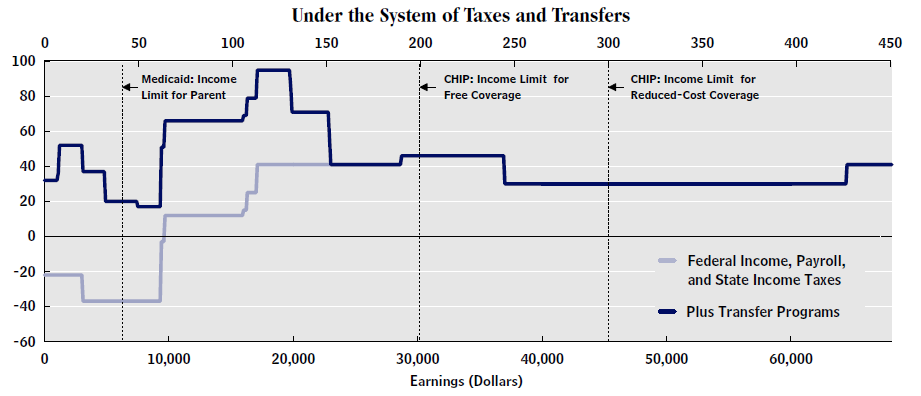
\includegraphics[width=.8\textwidth]{images/cbo-effective-tax-rate.png}
\end{center}
\caption{Effective Tax Rates. These are the effective tax rates computed by the
Congressional Budget Office in the United States.}
\label{fig:cbo-effective-tax-rate}
\end{figure}

\section{Simpler, Flatter, Fairer}

Flat taxes have got a bad reputation as being unfair. To a large extent, this
stems from a misunderstanding of what a flat tax is. What is flat is not the
\emph{average}, but rather the \emph{marginal} tax rate.

This may seem complicated, but what you want to have is a system where a
certain amount of your earnings are tax-free. Reasonable values may be \$10,000
for an individual (and \$20,000 for a couple filing jointly).\footnote{Having
limits applying to couples be double of those of individuals eliminates what is
sometimes called \emph{the marriage penalty}. This penalty comes from the way
in which the American tax system is structured. It penalizes marriage when both
members of the couple work and, in many cases, it even makes it
\emph{profitable for couples to divorce}! It is not opposed by republicans, for
all their bluster about being \emph{pro-family}. Nor is it opposed by
democrats, who might have been expected to object to the fact that this penalty
applies mostly to two-income households and so weighs against women working
when their husbands already do (of course, legally, it is the same whether it
is the husband who stays home while the wife makes a good living; but,
culturally, it is the woman who is more likely to feel pressure to stay home if
it is unprofitable for the couple).}

If we add a large deductable, we get a tax-system which \emph{is more
progressive than the current one}.

Harvard economist Greg Mankiw has argued that the current systems is, in fact
if not in spirit, a flat tax system.
% http://gregmankiw.blogspot.pt/2012/11/the-us-has-flat-tax-in-effect.html
In fact, if we look at Figure~\ref{fig:cbo-effective-tax-rate}, we realize that
the \emph{United States has a \textbf{regressive} tax system}: people on the
lower income scales face higher marginal rates than the upper middle class and
even high-incomes.

The only problem with this proposal is that it is politically naïve. The
argument goes something like the following: it will never pass in the United
States, where thousands of interest groups each enjoy their small benefit.
However, at some point in the not-so-distant future, the tax system will need
to change so that it collects more money. At that time, change will come. We
can only try to put good ideas out there so that they may then get picked up,
instead of the idea that was seriously discussed in January 2013 of minting a
trillion dollar coin.\footnote{I actually think it might have been a good idea
to mint that coin as a type of monetary policy, but why not do it properly
through a more active role for monetary policy coming from the Federal
Reserve?}

In Sweden, for most people, taxes are precomputed by the government based on
information provided by others (your employer and financial institutions).
Then, the government sends you their estimate. You have the option of just
accepting it or submitting your own tax information. Of course, small business
owners or those who freelance and have many clients may need to file
separately, but for over 90\% of people, the government's estimate will be
acceptable. The result is that the time it takes to do your taxes is about
30~minutes or less. Remember, doing taxes is a tax too.\footnote{How many hours
are wasted on this activity? Even with software like Turbo Tax (which itself
charges a small fee), too much effort is spent on taxes instead of productive
activity.}% FIXME: Actually look this up, are there estimates?

Finally, remember, it is not always about whether we should have the perfect
system or the current one. Removing even part of the complexity would be a
positive step forward.

\subsection{Simpler}

There are those people whose earnings are complex: they may be freelancers who
work in several states, have some moderate investment income, and rental
properties. For most of us, though, we have a single employer throughout the
year, wages are our main source of income, and any investment income is through
some managing institution (pension fund, bank, or such). At the end of year,
the government should be able to know how much you owe.

\subsection{Tax Expenditures}

In Portuguese, there is a useful word for a significant concept: \emph{to
debudget}.\footnote{Originally, \emph{desorçamentar}. It was coined in a few
years ago to accuse the government of the time of using accounting tricks to
hide the true value of government debt.} You debudget when you find a way to
keep the cost off the books.

Tax expenditures are a massive exercise in debudgeting. They also allow
Republican politicians to talk small government while continuing state support
for large corporations.

Let us end all the deductions that are nothing but micro-management of the
economy.

\subsection{Pigovian Taxes}

We will discuss this further on the chapter on the Environment, but taxes on
carbon emissions can be better for both the environment and the economy than
the current cacophony of taxes.

\subsection{Thoughts on Taxes}

\thought Means testing is a form of taxing the middle-incomes.

\thought A good tax is one where the induced incentives are as positive as the
revenue the tax brings.

\thought Conservatives are right on how high marginal tax rates can be
damaging, but do not often stress that the highest rates are paid by low-income
people.

\thought Complexity is regressive.


